\chapter{Graph Algorithm}

\section{Definitions}
A \textbf{graph} is an important mathematical structure. A graph \(G = (V, E)\) consists of a set of vertices (or nodes) \(V\) and a set of edges \(E\). Each edge is a pair \((v, w)\), where \(v, w \in V\). Edges are sometimes referred to as \textit{arcs}.

If \(e = (v, w)\) is an edge with vertices \(v\) and \(w\), then \(v\) and \(w\) are said to \textit{lie on} \(e\), and \(e\) is said to be \textit{incident with} \(v\) and \(w\).

If the pairs are unordered, then \(G\) is called an \textbf{undirected graph}. If the pairs are ordered, then \(G\) is called a \textbf{directed graph}. The term \textit{directed graph} is often shortened to \textit{digraph}, and the unqualified term \textit{graph} usually refers to an undirected graph.

Vertex \(w\) is said to be \textit{adjacent to} vertex \(v\) if and only if \((v, w) \in E\). In an undirected graph, if \((v, w) \in E\), then \((w, v) \in E\) as well, so \(v\) is adjacent to \(w\) and \(w\) is adjacent to \(v\). Sometimes, an edge has a third component, known as either a \textit{weight} or a \textit{cost}.

A \textbf{path} in a graph is a sequence of vertices \(w_1, w_2, \ldots, w_n\) such that \((w_i, w_{i+1}) \in E\) for \(1 \leq i \leq n - 1\). The \textit{length} of such a path is the number of edges on the path, which is equal to \(n - 1\). 

We allow a path from a vertex to itself. If this path contains no edges, then the path length is 0. If the graph contains an edge \((v, v)\) from a vertex to itself, then the path \(v, v\) is sometimes referred to as a \textbf{loop}. 

A \textbf{simple path} is a path in which all vertices are distinct, except that the first and last vertices may be the same.

A cycle in a directed graph is a path of length at least 1 such that \(w_1 = w_n\). This cycle is called *simple* if the path is simple. For undirected graphs, we require that the edges be distinct. The logic behind this requirement is that the path \(u, v, u\) in an undirected graph should not be considered a cycle, because \((u, v)\) and \((v, u)\) represent the same edge. However, in a directed graph, these are different edges, so it makes sense to call this a cycle.

A directed graph is acyclic if it has no cycles. A directed acyclic graph is sometimes referred to by its abbreviation, DAG.

An undirected graph is connected if there is a path from every vertex to every other vertex. A directed graph with this property is called strongly connected. If a directed graph is not strongly connected, but the underlying graph (without direction to the arcs) is connected, then the graph is said to be weakly connected. A complete graph is a graph in which there is an edge between every pair of vertices.

\section{Implementation}
Consider each airport as a vertex, and two vertices are connected by an edge if there is a nonstop flight between the airports represented by the vertices. The edge could have a weight, representing the time, distance, or cost of the flight. Such a graph is directed, since it might take longer or cost more to fly in different directions.

We would like to make sure that the airport system is strongly connected, so that it is always possible to fly from any airport to any other airport. We might also like to quickly determine the best flight between any two airports. This could mean the path with the fewest number of edges or could be taken with respect to one or all of the weight measures.

To implement such a system, we can use a \textbf{two-dimensional array}. This is known as an \textbf{adjacency matrix representation}. For each \textbf{edge} \((u, v)\), we set \(a[u][v] = 1\), otherwise the entry in the array is 0. If the edge has a \textbf{weight} associated with it, then we can set \(a[u][v]\) equal to the weight and use either a very large or a very small weight as a \textbf{sentinel} to indicate \textbf{nonexistent edges}.

Then, if we were looking for the cheapest airplane route, we could represent nonexistent flights with a cost of \(\infty\). If we were somehow looking for the most expensive airplane route, we could use \(-\infty\) to represent nonexistent edges.

The space requirement is \(\Theta(\vert V \vert^2)\). This is unacceptable if the graph does not have many edges. An adjacency matrix is an appropriate representation if the graph is dense, \(\vert E \vert = \Theta(\vert V \vert^2)\).

However, if the graph is not dense but sparse, a better solution is an adjacency list representation. For each vertex, we keep a list of all adjacent vertices. The space requirement is then \(O(\vert E \vert + \vert V \vert)\). If the edges have weights, then this additional information is also stored in the cells. 

\section{Topological Sort}
A \textbf{topological sort} is a \textbf{linear ordering of vertices} in a \textbf{directed acyclic graph (DAG)} such that for every directed edge from vertex \(u\) to vertex \(v\), vertex \(u\) comes before vertex \(v\) in the ordering. A directed edge \((v, w)\) indicates that course \(v\) must be completed before course \(w\) may be attempted.

A topological ordering is then a linear sequence of the vertices such that for every directed edge from vertex \(u\) to vertex \(v\), \(u\) appears before \(v\) in the sequence. In other words, the ordering respects all the directed dependencies in the graph.

Notice that a topological ordering is not possible with a cyclic graph, since for two vertices \(v\) and \(w\) on the cycle, \(v\) precedes \(w\) and \(w\) precedes \(v\). The ordering is not necessarily unique; any valid ordering will suffice.

To find the topological ordering, we first define the \textbf{in-degree} of a vertex \(v\) as the number of incoming edges \((u, v)\). We compute the in-degrees of all vertices in the graph. Then, we find any vertex with an in-degree of zero, print this vertex, and remove it along with its outgoing edges from the graph. We then apply this same strategy to the rest of the graph. 

\begin{minipage}{0.5\textwidth}
  \begin{figure}[H]
    \centering
    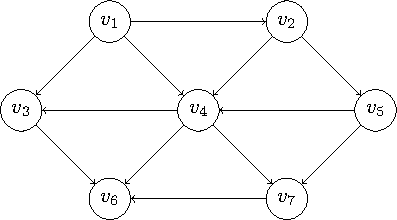
\includegraphics[width=0.8\textwidth]{Figure/topo_sort_demo.pdf}
    \caption{Topological Sort}
  \end{figure}
\end{minipage}
\begin{minipage}{0.5\textwidth}
  \begin{table}[H]
    \centering
    \begin{tabular}{c|c c c c c c c}
        \toprule
         & \multicolumn{7}{c}{In-degree before dequeue}  \\
      \midrule
        Vertex & 1 & 2 & 3 & 4 & 5 & 6 & 7  \\
      \midrule
        \(v_1\) & 0 & 0 & 0 & 0 & 0 & 0 & 0  \\
        \(v_2\) & 1 & 0 & 0 & 0 & 0 & 0 & 0  \\
        \(v_3\) & 2 & 1 & 1 & 1 & 0 & 0 & 0  \\
        \(v_4\) & 3 & 2 & 1 & 0 & 0 & 0 & 0  \\
        \(v_5\) & 1 & 1 & 0 & 0 & 0 & 0 & 0  \\
        \(v_6\) & 3 & 3 & 3 & 3 & 2 & 1 & 0  \\
        \(v_7\) & 2 & 2 & 2 & 1 & 0 & 0 & 0  \\
      \midrule
        \verb|enqueue| & \(v_1\) & \(v_2\) & \(v_5\) & \(v_4\) & \(v_3\) & \(v_7\) & \(v_6\)  \\
      \midrule
        \verb|dequeue| & \(v_1\) & \(v_2\) & \(v_5\) & \(v_4\) & \(v_3\) & \(v_7\) & \(v_6\)  \\
        \bottomrule
    \end{tabular}
    \caption{Topological Sorting}
  \end{table}
\end{minipage}

Since it is a simple sequential scan of the in-degree array, each call to it takes \(O(\vert V \vert)\) time. Since there are \(\vert V \vert\) such calls, the running time of the algorithm is \(O(\vert V \vert^2)\).

\section{Algorithms}
Here we introduce some algorithms that are related to graphs.

\subsection{Shortest Path Algorithm}
For the shortest path algorithm, the input is a weighted graph. Associated with each edge \((v_i, v_j)\) is a cost \(c_{i, j}\) to traverse the arc. The cost of a path \(v_1, v_2, \cdots, v_n\) is \(\sum_{i = 1}^{n - 1} c_{i, i + 1}\). This is referred to as the weighted path length. The unweighted path length is merely the number of edges on the path, namely \(n - 1\).

\begin{minipage}{0.5\textwidth}
  \begin{figure}[H]
    \centering
    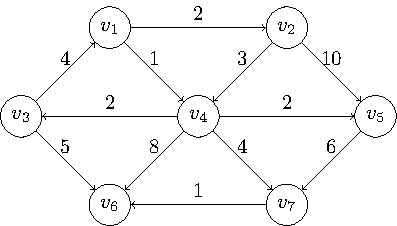
\includegraphics[width=0.7\textwidth]{Figure/shortest_path_algo.pdf}
    \caption{A weighted graph}
  \end{figure}
\end{minipage}\quad\quad
\begin{minipage}{0.5\textwidth}
  \begin{figure}[H]
    \centering
    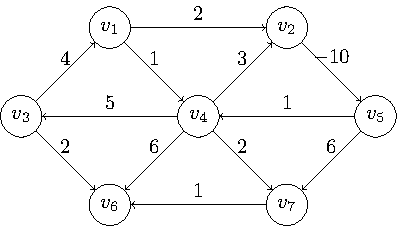
\includegraphics[width=0.7\textwidth]{Figure/ng_weight_path.pdf}
    \caption{A weighted graph}
  \end{figure}
\end{minipage}\quad\quad

For example, given as input a weighted graph \(G = (V, E)\) and a distinguished vertex \(s\), we are asked to find the shortest weighted path from \(s\) to every other vertex in \(G\).

In Figure 9.2, the shortest weighted path from \(v_1\) to \(v_6\) has a cost of 6 and goes from \(v_1\) to \(v_4\) to \(v_7\) to \(v_6\). The shortest unweighted path between these vertices has a length of 2. 

There could also be cases where the cost is negative. For example, in Figure 9.3, the path from \(v_5\) to \(v_4\) has cost 1, but a shorter path exists by following the loop \(v_5, v_4, v_2, v_5, v_4\), which has a cost of \(-5\). The shortest path between \(v_5\) and \(v_4\) is undefined. This loop is known as a negative-cost cycle. When one is present in the graph, the shortest paths are not defined.

Currently, there are no algorithms in which finding the path from \(s\) to one vertex is significantly faster (by more than a constant factor) than finding the paths from \(s\) to all vertices. The intermediate nodes in a shortest path must also lie on the shortest paths from \(s\).

If we assume that there are no negative edges, then for the weighted shortest path problem, the running time of the algorithm will be \(O(\vert E \vert \log \vert V \vert)\) when implemented with reasonable data structures.

If the graph has negative edges, we will have a poor time bound of \(O(\vert E \vert \cdot \vert V \vert)\). We will solve the weighted problem for the special case of acyclic graphs in linear time.

\subsection{Breadth-First Search}
We want to find the unweighted shortest path. Using vertex \(s\), we would like to find the shortest path from \(s\) to all other vertices. There are no weights on the edges, which is a special case of the weighted shortest-path problem, since we could assign all edges a weight of 1. 

We can use \textbf{breadth-first search (BFS)} to search for the shortest path. It operates by processing vertices in layers. The vertices closest to the start are evaluated first, and the most distant vertices are evaluated last. This is much the same as a level-order traversal for trees.



For each vertex, we will keep track of three pieces of information. First, we will keep its distance from \(s\) in the entry \(d_v\). Initially, all vertices are unreachable except for \(s\), whose path length is 0. The entry in \(p_v\) is the bookkeeping variable, which will allow us to print the actual paths. The entry \texttt{known} is set to 1 after a vertex is processed. Initially, all entries are unknown, including the start vertex. Once it is known, we have a guarantee that no cheaper path will ever be found, and so processing for that vertex is essentially complete.

In Figure 9.4, suppose we choose \(s\) to be \(v_3\). The shortest path from \(s\) to \(v_3\) is then a path of length 0. Now we can start looking for all vertices that are a distance 1 away from \(s\). These can be found by looking at the vertices that are adjacent to \(s\). Then we have

\begin{minipage}{0.33\textwidth}
  \begin{figure}[H]
    \centering
    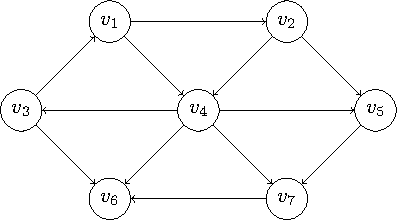
\includegraphics[width=\textwidth]{Figure/unweighted_path.pdf}
    \caption{Unweighted graph}
  \end{figure}
\end{minipage}
\begin{minipage}{0.33\textwidth}
\begin{table}[H]
  \centering
  \begin{tabular}{c|c|c|c}
      \toprule
      \verb|v| & Known & \(d_v\) & \(p_v\)  \\
    \midrule
      \(v_1\) & 0 & \(\infty\) & 0  \\
      \(v_2\) & 0 & \(\infty\) & 0  \\
      \(v_3\) & 0 & \(0\) & 0  \\
      \(v_4\) & 0 & \(\infty\) & 0  \\
      \(v_5\) & 0 & \(\infty\) & 0  \\
      \(v_6\) & 0 & \(\infty\) & 0  \\
      \(v_7\) & 0 & \(\infty\) & 0  \\
    \midrule
      \verb|Q| & \multicolumn{3}{c}{\(v_3\)} \\
    \bottomrule
  \end{tabular}
  \caption*{Initial State}
\end{table}
\end{minipage}
\begin{minipage}{0.33\textwidth}
  \begin{table}[H]
    \centering
    \begin{tabular}{c|c|c|c}
        \toprule
        \verb|v| & Known & \(d_v\) & \(p_v\)  \\
      \midrule
        \(v_1\) & 0 & 1 & \(v_3\)  \\
        \(v_2\) & 0 & \(\infty\) & 0  \\
        \(v_3\) & 1 & 0 & 0  \\
        \(v_4\) & 0 & \(\infty\) & 0  \\
        \(v_5\) & 0 & \(\infty\) & 0  \\
        \(v_6\) & 0 & 1 & \(v_3\)  \\
        \(v_7\) & 0 & \(\infty\) & 0  \\
      \midrule
        \verb|Q| & \multicolumn{3}{c}{\(v_1, v_6\)} \\
      \bottomrule
    \end{tabular}
    \caption*{\(v_3\) dequeued}
  \end{table}
\end{minipage}

\begin{minipage}{0.33\textwidth}
  \begin{table}[H]
    \centering
    \begin{tabular}{c|c|c|c}
        \toprule
        \verb|v| & Known & \(d_v\) & \(p_v\)  \\
      \midrule
        \(v_1\) & 1 & 1 & \(v_3\)  \\
        \(v_2\) & 0 & 2 & \(v_1\)  \\
        \(v_3\) & 1 & 0 & 0  \\
        \(v_4\) & 0 & 2 & \(v_1\)  \\
        \(v_5\) & 0 & \(\infty\) & 0  \\
        \(v_6\) & 0 & 1 & \(v_3\)  \\
        \(v_7\) & 0 & \(\infty\) & 0  \\
      \midrule
        \verb|Q| & \multicolumn{3}{c}{\(v_6, v_2, v_4\)} \\
      \bottomrule
    \end{tabular}
    \caption*{\(v_1\) dequeued}
  \end{table}
\end{minipage}
\begin{minipage}{0.33\textwidth}
  \begin{table}[H]
    \centering
    \begin{tabular}{c|c|c|c}
        \toprule
        \verb|v| & Known & \(d_v\) & \(p_v\)  \\
      \midrule
        \(v_1\) & 1 & 1 & \(v_3\)  \\
        \(v_2\) & 0 & 2 & \(v_1\)  \\
        \(v_3\) & 1 & 0 & 0  \\
        \(v_4\) & 0 & 2 & \(v_1\)  \\
        \(v_5\) & 0 & \(\infty\) & 0  \\
        \(v_6\) & 1 & 1 & \(v_3\)  \\
        \(v_7\) & 0 & \(\infty\) & 0  \\
      \midrule
        \verb|Q| & \multicolumn{3}{c}{\(v_2, v_4\)} \\
      \bottomrule
    \end{tabular}
    \caption*{\(v_6\) dequeued}
  \end{table}
\end{minipage}
\begin{minipage}{0.33\textwidth}
  \begin{table}[H]
    \centering
    \begin{tabular}{c|c|c|c}
        \toprule
        \verb|v| & Known & \(d_v\) & \(p_v\)  \\
      \midrule
        \(v_1\) & 1 & 1 & \(v_3\)  \\
        \(v_2\) & 1 & 2 & \(v_1\)  \\
        \(v_3\) & 1 & 0 & 0  \\
        \(v_4\) & 0 & 2 & \(v_1\)  \\
        \(v_5\) & 0 & 3 & \(v_2\)   \\
        \(v_6\) & 1 & 1 & \(v_3\)  \\
        \(v_7\) & 0 & \(\infty\) & 0  \\
      \midrule
        \verb|Q| & \multicolumn{3}{c}{\(v_4, v_5\)} \\
      \bottomrule
    \end{tabular}
    \caption*{\(v_2\) dequeued}
  \end{table}
\end{minipage}

\begin{minipage}{0.33\textwidth}
  \begin{table}[H]
    \centering
    \begin{tabular}{c|c|c|c}
        \toprule
        \verb|v| & Known & \(d_v\) & \(p_v\)  \\
      \midrule
        \(v_1\) & 1 & 1 & \(v_3\)  \\
        \(v_2\) & 1 & 2 & \(v_1\)  \\
        \(v_3\) & 1 & 0 & 0  \\
        \(v_4\) & 1 & 2 & \(v_1\)  \\
        \(v_5\) & 0 & 3 & \(v_2\)   \\
        \(v_6\) & 1 & 1 & \(v_3\)  \\
        \(v_7\) & 0 & 3 & \(v_4\)  \\
      \midrule
        \verb|Q| & \multicolumn{3}{c}{\(v_5, v_7\)} \\
      \bottomrule
    \end{tabular}
    \caption*{\(v_4\) dequeued}
  \end{table}
\end{minipage}
\begin{minipage}{0.33\textwidth}
  \begin{table}[H]
    \centering
    \begin{tabular}{c|c|c|c}
        \toprule
        \verb|v| & Known & \(d_v\) & \(p_v\)  \\
      \midrule
        \(v_1\) & 1 & 1 & \(v_3\)  \\
        \(v_2\) & 1 & 2 & \(v_1\)  \\
        \(v_3\) & 1 & 0 & 0  \\
        \(v_4\) & 1 & 2 & \(v_1\)  \\
        \(v_5\) & 1 & 3 & \(v_2\)   \\
        \(v_6\) & 1 & 1 & \(v_3\)  \\
        \(v_7\) & 0 & 3 & \(v_4\)  \\
      \midrule
        \verb|Q| & \multicolumn{3}{c}{\(v_7\)} \\
      \bottomrule
    \end{tabular}
    \caption*{\(v_5\) dequeued}
  \end{table}
\end{minipage}
\begin{minipage}{0.33\textwidth}
  \begin{table}[H]
    \centering
    \begin{tabular}{c|c|c|c}
        \toprule
        \verb|v| & Known & \(d_v\) & \(p_v\)  \\
      \midrule
        \(v_1\) & 1 & 1 & \(v_3\)  \\
        \(v_2\) & 1 & 2 & \(v_1\)  \\
        \(v_3\) & 1 & 0 & 0  \\
        \(v_4\) & 1 & 2 & \(v_1\)  \\
        \(v_5\) & 1 & 3 & \(v_2\)   \\
        \(v_6\) & 1 & 1 & \(v_3\)  \\
        \(v_7\) & 1 & 3 & \(v_4\)  \\
      \midrule
        \verb|Q| & \multicolumn{3}{c}{} \\
      \bottomrule
    \end{tabular}
    \caption*{\(v_7\) dequeued}
  \end{table}
\end{minipage}

The running time for this algorithm is \(O(\vert V \vert^2)\), because of the doubly nested \texttt{for} loops.

\subsection{Dijkstra's Algorithm}
If the graph is weighted, the problem becomes harder. However, we can still use the idea from the unweighted case.

Again, each vertex is marked as either known or unknown. A tentative distance \(d_v\) is kept for each vertex, as before. This distance turns out to be the shortest path length from \(s\) to \(v\) using only known vertices as intermediates. As before, we record \(p_v\), which is the last vertex to cause a change to \(d_v\).

The general method to solve the single-source shortest-path problem is known as Dijkstra's algorithm. This is a prime example of a greedy algorithm. Greedy algorithms generally solve a problem in stages by doing what appears to be the best choice at each stage.

Notice that Dijkstra's algorithm proceeds in stages. At each stage, Dijkstra's algorithm selects a vertex \(v\), which has the smallest \(d_v\) among all the unknown vertices, and declares that the shortest path from \(s\) to \(v\) is known. The remainder of a stage consists of updating the values of \(d_w\).

Consider the following example:

\begin{minipage}{0.33\textwidth}
  \begin{figure}[H]
    \centering
    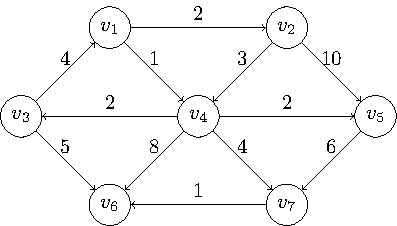
\includegraphics[width=\textwidth]{Figure/shortest_path_algo.pdf}
    \caption{A weighted graph}
  \end{figure}
\end{minipage}\quad\quad
\begin{minipage}{0.33\textwidth}
\begin{table}[H]
  \centering
  \begin{tabular}{c|c|c|c}
      \toprule
      \verb|v| & Known & \(d_v\) & \(p_v\)  \\
    \midrule
      \(v_1\) & 0 & 0 & 0  \\
      \(v_2\) & 0 & \(\infty\) & 0  \\
      \(v_3\) & 0 & \(\infty\) & 0  \\
      \(v_4\) & 0 & \(\infty\) & 0  \\
      \(v_5\) & 0 & \(\infty\) & 0  \\
      \(v_6\) & 0 & \(\infty\) & 0  \\
      \(v_7\) & 0 & \(\infty\) & 0  \\
    \bottomrule
  \end{tabular}
  \caption*{Initial State}
\end{table}
\end{minipage}
\begin{minipage}{0.33\textwidth}
\begin{table}[H]
  \centering
  \begin{tabular}{c|c|c|c}
      \toprule
      \verb|v| & Known & \(d_v\) & \(p_v\)  \\
    \midrule
      \(v_1\) & 1 & 0 & 0  \\
      \(v_2\) & 0 & 2 & \(v_1\)  \\
      \(v_3\) & 0 & \(\infty\) & 0  \\
      \(v_4\) & 0 & 1 & \(v_1\)  \\
      \(v_5\) & 0 & \(\infty\) & 0  \\
      \(v_6\) & 0 & \(\infty\) & 0  \\
      \(v_7\) & 0 & \(\infty\) & 0  \\
    \bottomrule
  \end{tabular}
  \caption*{After \(v_1\)}
\end{table}
\end{minipage}

\begin{minipage}{0.33\textwidth}
\begin{table}[H]
  \centering
  \begin{tabular}{c|c|c|c}
      \toprule
      \verb|v| & Known & \(d_v\) & \(p_v\)  \\
    \midrule
      \(v_1\) & 1 & 0 & 0  \\
      \(v_2\) & 0 & 2 & \(v_1\)  \\
      \(v_3\) & 0 & 3 & \(v_4\)  \\
      \(v_4\) & 1 & 1 & \(v_1\)  \\
      \(v_5\) & 0 & 3 & \(v_4\)  \\
      \(v_6\) & 0 & 9 & \(v_4\)  \\
      \(v_7\) & 0 & 5 & \(v_4\)  \\
    \bottomrule
  \end{tabular}
  \caption*{After \(v_4\)}
\end{table}
\end{minipage}
\begin{minipage}{0.33\textwidth}
\begin{table}[H]
  \centering
  \begin{tabular}{c|c|c|c}
      \toprule
      \verb|v| & Known & \(d_v\) & \(p_v\)  \\
    \midrule
      \(v_1\) & 1 & 0 & 0  \\
      \(v_2\) & 1 & 2 & \(v_1\)  \\
      \(v_3\) & 0 & 3 & \(v_4\)  \\
      \(v_4\) & 1 & 1 & \(v_1\)  \\
      \(v_5\) & 0 & 3 & \(v_4\)  \\
      \(v_6\) & 0 & 9 & \(v_4\)  \\
      \(v_7\) & 0 & 5 & \(v_4\)  \\
    \bottomrule
  \end{tabular}
  \caption*{After \(v_2\)}
\end{table}
\end{minipage}
\begin{minipage}{0.33\textwidth}
  \begin{table}[H]
    \centering
    \begin{tabular}{c|c|c|c}
        \toprule
        \verb|v| & Known & \(d_v\) & \(p_v\)  \\
      \midrule
        \(v_1\) & 1 & 0 & 0  \\
        \(v_2\) & 1 & 2 & \(v_1\)  \\
        \(v_3\) & 1 & 3 & \(v_4\)  \\
        \(v_4\) & 1 & 1 & \(v_1\)  \\
        \(v_5\) & 1 & 3 & \(v_4\)  \\
        \(v_6\) & 0 & 8 & \(v_3\)  \\
        \(v_7\) & 0 & 5 & \(v_4\)  \\
      \bottomrule
    \end{tabular}
    \caption*{After \(v_3\) and \(v_5\)}
  \end{table}
\end{minipage}

\begin{minipage}{0.5\textwidth}
  \begin{table}[H]
    \centering
    \begin{tabular}{c|c|c|c}
        \toprule
        \verb|v| & Known & \(d_v\) & \(p_v\)  \\
      \midrule
        \(v_1\) & 1 & 0 & 0  \\
        \(v_2\) & 1 & 2 & \(v_1\)  \\
        \(v_3\) & 1 & 3 & \(v_4\)  \\
        \(v_4\) & 1 & 1 & \(v_1\)  \\
        \(v_5\) & 1 & 3 & \(v_4\)  \\
        \(v_6\) & 0 & 6 & \(v_7\)  \\
        \(v_7\) & 1 & 5 & \(v_4\)  \\
      \bottomrule
    \end{tabular}
    \caption*{After \(v_7\)}
  \end{table}
\end{minipage}
\begin{minipage}{0.5\textwidth}
  \begin{table}[H]
    \centering
    \begin{tabular}{c|c|c|c}
        \toprule
        \verb|v| & Known & \(d_v\) & \(p_v\)  \\
      \midrule
        \(v_1\) & 1 & 0 & 0  \\
        \(v_2\) & 1 & 2 & \(v_1\)  \\
        \(v_3\) & 1 & 3 & \(v_4\)  \\
        \(v_4\) & 1 & 1 & \(v_1\)  \\
        \(v_5\) & 1 & 3 & \(v_4\)  \\
        \(v_6\) & 1 & 6 & \(v_7\)  \\
        \(v_7\) & 1 & 5 & \(v_4\)  \\
      \bottomrule
    \end{tabular}
    \caption*{After \(v_6\)}
  \end{table}
\end{minipage}

However, Dijkstra's algorithm does not work with negative edge costs. A combination of the weighted and unweighted algorithms will solve the problem, but at the cost of a drastic increase in running time. The running time is \(O(\vert E \vert \cdot \vert V \vert)\) if adjacency lists are used.

We can improve this algorithm by changing the order in which vertices are declared known, otherwise known as the vertex selection rule. The new rule is to select vertices in topological order. The algorithm can be done in one pass, since the selections and updates can take place as the topological sort is being performed.

The selection rule works because when a vertex \(v\) is selected, its distance \(d_v\) can no longer be lowered. Since, by the topological ordering rule, it has no incoming edges emanating from unknown nodes, the running time is \(O(\vert E \vert + \vert V \vert)\), since the selection takes constant time.

There are several applications, including the downhill skiing problem, modeling of chemical reactions, and critical path analysis. For critical path analysis, each node represents an activity that must be performed, along with the time it takes to complete the activity. This graph is thus known as an activity-node graph.

For an activity-node graph, the edges represent precedence relationships. An edge \((v, w)\) means that activity \(v\) must be completed before activity \(w\) may begin. This implies that the graph must be acyclic.

If we need to find the shortest paths between all pairs of vertices in the graph, a brute-force method is to run the appropriate single-source algorithm \(\vert V \vert\) times. On sparse graphs, it is faster to run \(\vert V \vert\) Dijkstra's algorithms coded with priority queues.

\section{Maximum-Flow Algorithm}
Suppose we are given a directed graph \(G = (V, E)\) with edge capacities \(c_{v, w}\). These capacities could represent the amount of water that can flow through a pipe or the amount of traffic that can flow on a street between two intersections. We have two vertices: \(s\), which we call the source, and \(t\), which is the sink. Through any edge \((v, w)\), at most \(c_{v, w}\) units of ``flow'' may pass.

For any vertex \(v\) that is neither \(s\) nor \(t\), the total flow coming in must equal the total flow going out. The maximum flow problem is to determine the maximum amount of flow that can pass from \(s\) to \(t\).

To solve this problem, we can use a simple maximum-flow algorithm. We have \(G_f\) as a flow graph, which represents the flow that has been attained at any stage in the algorithm. Initially, all edges in \(G_f\) have no flow. \(G_f\) should contain a maximum flow when the algorithm terminates.

We also have \(G_r\), the residual graph. \(G_r\) tells, for each edge, how much more flow can be added. We calculate this by subtracting the current flow from the capacity for each edge. An edge in \(G_r\) is known as a residual edge.

At each stage, we find a path in \(G_r\) from \(s\) to \(t\). This path is known as an augmenting path. The minimum edge on this path determines the amount of flow that can be added to every edge on the path. We do this by adjusting \(G_f\) and recomputing \(G_r\). When we find no path from \(s\) to \(t\) in \(G_r\), we terminate. This algorithm is nondeterministic in that we are free to choose any path from \(s\) to \(t\).

Consider the following example: 

\begin{minipage}{0.2\textwidth}
\begin{figure}[H]
  \centering
  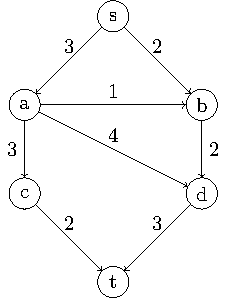
\includegraphics[width=0.8\textwidth]{Figure/maxflow_d1_1.pdf}
  \caption*{Initial Stage \(G\)}
\end{figure}
\end{minipage}
\begin{minipage}{0.2\textwidth}
\begin{figure}[H]
  \centering
  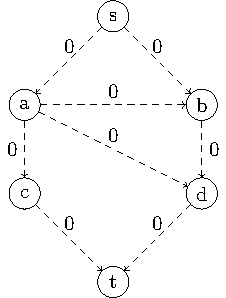
\includegraphics[width=0.8\textwidth]{Figure/maxflow_d1_2.pdf}
  \caption*{1 Flow Graph \(G_f\)}
\end{figure}
\end{minipage}
\begin{minipage}{0.2\textwidth}
\begin{figure}[H]
  \centering
  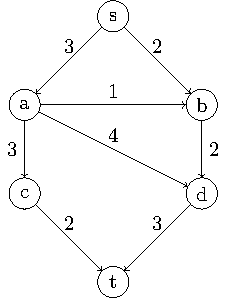
\includegraphics[width=0.8\textwidth]{Figure/maxflow_d1_3.pdf}
  \caption*{1 Residual Graph \(G_r\)}
\end{figure}
\end{minipage}
\begin{minipage}{0.2\textwidth}
\begin{figure}[H]
  \centering
  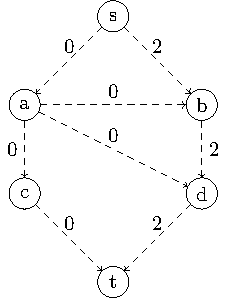
\includegraphics[width=0.8\textwidth]{Figure/maxflow_d1_4.pdf}
  \caption*{2 Flow Graph \(G_f\)}
\end{figure}
\end{minipage}
\begin{minipage}{0.2\textwidth}
\begin{figure}[H]
  \centering
  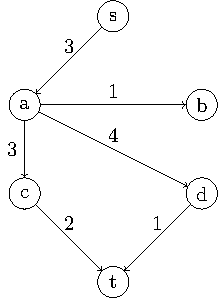
\includegraphics[width=0.8\textwidth]{Figure/maxflow_d1_5.pdf}
  \caption*{2 Residual Graph \(G_r\)}
\end{figure}
\end{minipage}

\begin{minipage}{0.2\textwidth}
\begin{figure}[H]
  \centering
  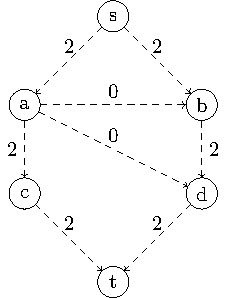
\includegraphics[width=0.8\textwidth]{Figure/maxflow_d1_6.pdf}
  \caption*{3 Flow Graph \(G_f\)}
\end{figure}
\end{minipage}
\begin{minipage}{0.2\textwidth}
\begin{figure}[H]
  \centering
  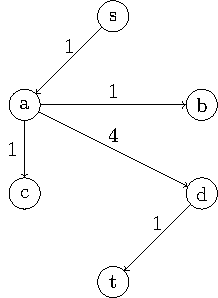
\includegraphics[width=0.8\textwidth]{Figure/maxflow_d1_7.pdf}
  \caption*{3 Residual Graph \(G_r\)}
\end{figure}
\end{minipage}
\begin{minipage}{0.2\textwidth}
\begin{figure}[H]
  \centering
  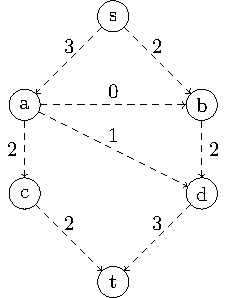
\includegraphics[width=0.8\textwidth]{Figure/maxflow_d1_8.pdf}
  \caption*{4 Flow Graph \(G_f\)}
\end{figure}
\end{minipage}
\begin{minipage}{0.2\textwidth}
\begin{figure}[H]
  \centering
  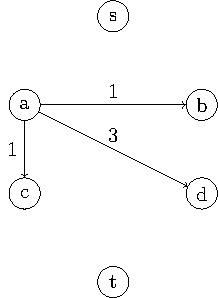
\includegraphics[width=0.8\textwidth]{Figure/maxflow_d1_9.pdf}
  \caption*{4 Residual Graph \(G_r\)}
\end{figure}
\end{minipage}

Starting from the initial stage, we add different units of flow according to the bottleneck. At the end, there is no more path from \(s\) to \(t\), and thus the algorithm terminates.

The resulting flow of 5 happens to be the maximum flow. However, this is not the optimal solution. Suppose we choose the path \(s, a, d, t\) as the initial path. Then, the result of this choice is that there is no longer any path from \(s\) to \(t\) in the residual graph.

We can optimize it by allowing the algorithm to change its mind. To do this, for every edge \((v, w)\) with flow \(f_{v, w}\) in the flow graph, we will add an edge in the residual graph \((w, v)\) with capacity \(f_{v, w}\). In effect, we are allowing the algorithm to undo its decisions by sending flow back in the opposite direction.

Consider the following example follows the same initial stage: 

\begin{minipage}{0.2\textwidth}
\begin{figure}[H]
  \centering
  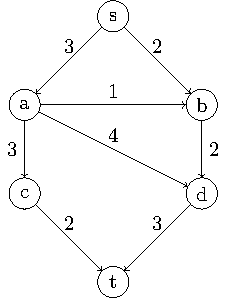
\includegraphics[width=0.8\textwidth]{Figure/maxflow_d2_1.pdf}
  \caption*{Initial Stage \(G\)}
\end{figure}
\end{minipage}
\begin{minipage}{0.2\textwidth}
\begin{figure}[H]
  \centering
  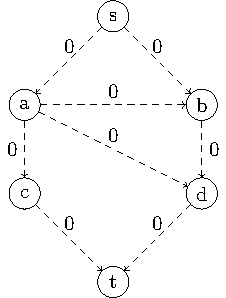
\includegraphics[width=0.8\textwidth]{Figure/maxflow_d2_2.pdf}
  \caption*{1 Flow Graph \(G_f\)}
\end{figure}
\end{minipage}
\begin{minipage}{0.2\textwidth}
\begin{figure}[H]
  \centering
  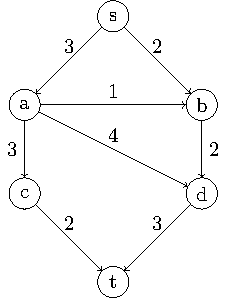
\includegraphics[width=0.8\textwidth]{Figure/maxflow_d2_3.pdf}
  \caption*{1 Residual Graph \(G_r\)}
\end{figure}
\end{minipage}
\begin{minipage}{0.2\textwidth}
\begin{figure}[H]
  \centering
  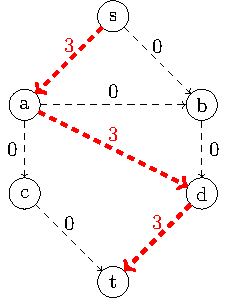
\includegraphics[width=0.8\textwidth]{Figure/maxflow_d2_4.pdf}
  \caption*{2 Flow Graph \(G_f\)}
\end{figure}
\end{minipage}
\begin{minipage}{0.2\textwidth}
\begin{figure}[H]
  \centering
  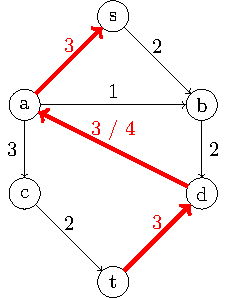
\includegraphics[width=0.8\textwidth]{Figure/maxflow_d2_5.pdf}
  \caption*{2 Residual Graph \(G_r\)}
\end{figure}
\end{minipage}

\begin{minipage}{0.2\textwidth}
\begin{figure}[H]
  \centering
  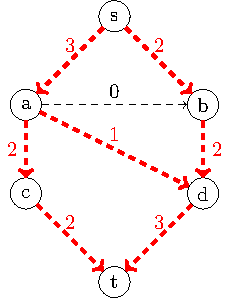
\includegraphics[width=0.8\textwidth]{Figure/maxflow_d2_6.pdf}
  \caption*{3 Flow Graph \(G_f\)}
\end{figure}
\end{minipage}
\begin{minipage}{0.2\textwidth}
\begin{figure}[H]
  \centering
  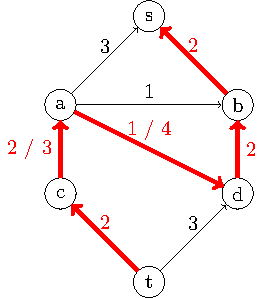
\includegraphics[width=0.8\textwidth]{Figure/maxflow_d2_7.pdf}
  \caption*{3 Residual Graph \(G_r\)}
\end{figure}
\end{minipage}

As seen from this flow, although we initially choose the path \(s, a, d, t\), in the residual graph, there are edges in both directions between \(a\) and \(d\). Either one more unit of flow can be pushed from \(a\) to \(d\), or up to three units can be pushed back—thus, we can undo flow. Now, the algorithm finds the augmenting path \(s, b, d, a, c, t\). By pushing two units of flow from \(d\) to \(a\), the algorithm removes two units of flow from the edge \((a, d)\), effectively changing its previous decision.

Notice that if the capacities are all integers and the maximum flow is \(f\), then since each augmenting path increases the flow value by at least 1, \(f\) stages suffice. The total running time is \(O(f \cdot \vert E \vert)\), since an augmenting path can be found in \(O(\vert E \vert)\) time using an unweighted shortest-path algorithm.

\begin{remark}
  We always choose the augmenting path that allows the largest increase in the flow. Finding such a path is similar to solving a weighted shortest-path problem.
\end{remark}

\section{Minimum Spanning Tree}
Informally, a \textit{minimum spanning tree} of an undirected graph \(G\) is a tree formed from graph edges that connects all the vertices of \(G\) at the lowest total cost. A minimum spanning tree exists if and only if \(G\) is connected.

The minimum spanning tree is unique only when all edge weights are distinct.

Note that the number of edges in a minimum spanning tree is \(\vert V \vert - 1\). It is a \textit{tree} because it is acyclic, \textit{spanning} because it covers all the vertices, and \textit{minimum} because the sum of the edge costs is the lowest possible.

We can construct a minimum spanning tree using \textbf{Prim's algorithm}, which grows the tree in successive stages. At each stage, starting from a root node, we add an edge—and thus an associated vertex—to the tree. The algorithm selects the edge \((u, v)\) with the smallest cost such that \(u\) is in the tree and \(v\) is not.

Prim's algorithm is essentially identical to Dijkstra's algorithm for shortest paths. For each vertex, we maintain values \(d_v\) and \(p_v\), as well as an indication of whether it is \textit{known} or \textit{unknown}.

Here, \(d_v\) is the weight of the shortest edge connecting \(v\) to any known vertex. The variable \(p_v\), as before, records the last vertex to cause a change in \(d_v\). After a vertex \(v\) is selected, for each unknown neighbor \(w\), we update:
\[
d_w = \min(d_w, c_{w,v})
\]

Consider the following example:

\begin{minipage}{0.25\textwidth}
\begin{figure}[H]
  \centering
  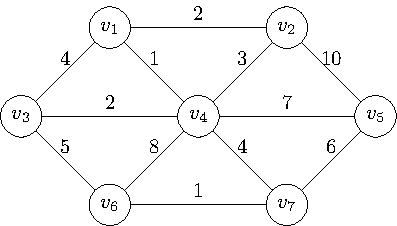
\includegraphics[width=0.8\textwidth]{Figure/min_span.pdf}
\end{figure}
\end{minipage}
\begin{minipage}{0.25\textwidth}
\begin{figure}[H]
  \centering
  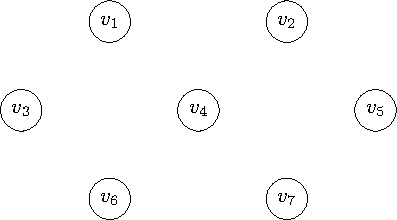
\includegraphics[width=0.8\textwidth]{Figure/prim_algo_d1.pdf}
\end{figure}
\end{minipage}
\begin{minipage}{0.25\textwidth}
\begin{figure}[H]
  \centering
  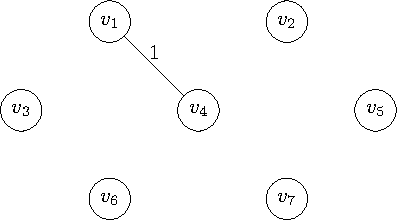
\includegraphics[width=0.8\textwidth]{Figure/prim_algo_d2.pdf}
\end{figure}
\end{minipage}
\begin{minipage}{0.25\textwidth}
\begin{figure}[H]
  \centering
  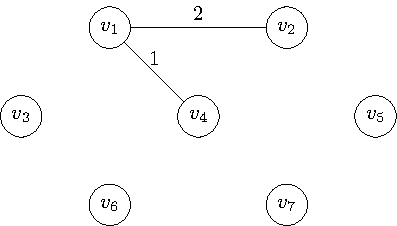
\includegraphics[width=0.8\textwidth]{Figure/prim_algo_d3.pdf}
\end{figure}
\end{minipage}

\begin{minipage}{0.25\textwidth}
\begin{figure}[H]
  \centering
  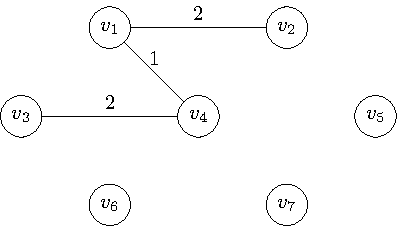
\includegraphics[width=0.8\textwidth]{Figure/prim_algo_d4.pdf}
\end{figure}
\end{minipage}
\begin{minipage}{0.25\textwidth}
\begin{figure}[H]
  \centering
  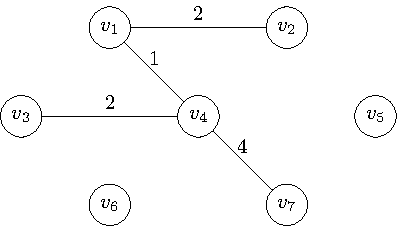
\includegraphics[width=0.8\textwidth]{Figure/prim_algo_d5.pdf}
\end{figure}
\end{minipage}
\begin{minipage}{0.25\textwidth}
\begin{figure}[H]
  \centering
  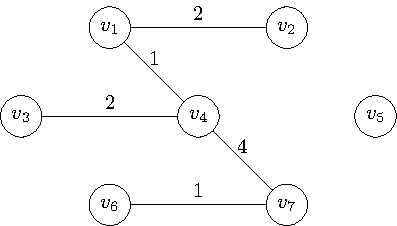
\includegraphics[width=0.8\textwidth]{Figure/prim_algo_d6.pdf}
\end{figure}
\end{minipage}
\begin{minipage}{0.25\textwidth}
\begin{figure}[H]
  \centering
  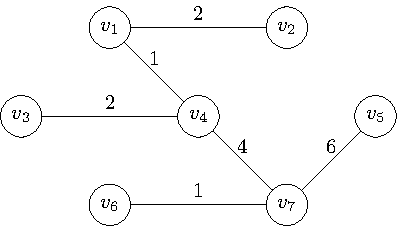
\includegraphics[width=0.8\textwidth]{Figure/prim_algo_d7.pdf}
\end{figure}
\end{minipage}

We can also use tables to show the results: 

\begin{minipage}{0.33\textwidth}
\begin{table}[H]
  \centering
  \begin{tabular}{c|c|c|c}
      \toprule
      \(v\) & Known & \(d_v\) & \(p_v\)  \\
    \midrule
      \(v_1\) & 0 & 0 & 0  \\
      \(v_2\) & 0 & \(\infty\) & 0  \\
      \(v_3\) & 0 & \(\infty\) & 0  \\
      \(v_4\) & 0 & \(\infty\) & 0  \\
      \(v_5\) & 0 & \(\infty\) & 0  \\
      \(v_6\) & 0 & \(\infty\) & 0  \\
      \(v_7\) & 0 & \(\infty\) & 0  \\
      \bottomrule
  \end{tabular}
  \caption*{Initial Stage}
\end{table}
\end{minipage}
\begin{minipage}{0.33\textwidth}
\begin{table}[H]
  \centering
  \begin{tabular}{c|c|c|c}
      \toprule
      \(v\) & Known & \(d_v\) & \(p_v\)  \\
    \midrule
      \(v_1\) & 1 & 0 & 0  \\
      \(v_2\) & 0 & 2 & \(v_1\)  \\
      \(v_3\) & 0 & 4 & \(v_1\)  \\
      \(v_4\) & 0 & 1 & \(v_1\)  \\
      \(v_5\) & 0 & \(\infty\) & 0  \\
      \(v_6\) & 0 & \(\infty\) & 0  \\
      \(v_7\) & 0 & \(\infty\) & 0  \\
      \bottomrule
  \end{tabular}
  \caption*{After \(v_1\)}
\end{table}
\end{minipage}
\begin{minipage}{0.33\textwidth}
\begin{table}[H]
  \centering
  \begin{tabular}{c|c|c|c}
      \toprule
      \(v\) & Known & \(d_v\) & \(p_v\)  \\
    \midrule
      \(v_1\) & 1 & 0 & 0  \\
      \(v_2\) & 0 & 2 & \(v_1\)  \\
      \(v_3\) & 0 & 2 & \(v_4\)  \\
      \(v_4\) & 1 & 1 & \(v_1\)  \\
      \(v_5\) & 0 & 7 & \(v_4\)  \\
      \(v_6\) & 0 & 8 & \(v_4\)  \\
      \(v_7\) & 0 & 4 & \(v_4\)  \\
      \bottomrule
  \end{tabular}
  \caption*{After \(v_4\)}
\end{table}
\end{minipage}

\begin{minipage}{0.33\textwidth}
\begin{table}[H]
  \centering
  \begin{tabular}{c|c|c|c}
      \toprule
      \(v\) & Known & \(d_v\) & \(p_v\)  \\
    \midrule
      \(v_1\) & 1 & 0 & 0  \\
      \(v_2\) & 1 & 2 & \(v_1\)  \\
      \(v_3\) & 1 & 2 & \(v_4\)  \\
      \(v_4\) & 1 & 1 & \(v_1\)  \\
      \(v_5\) & 0 & 7 & \(v_4\)  \\
      \(v_6\) & 0 & 5 & \(v_3\)  \\
      \(v_7\) & 0 & 4 & \(v_4\)  \\
      \bottomrule
  \end{tabular}
  \caption*{After \(v_2\) and \(v_3\)}
\end{table}
\end{minipage}
\begin{minipage}{0.33\textwidth}
\begin{table}[H]
  \centering
  \begin{tabular}{c|c|c|c}
      \toprule
      \(v\) & Known & \(d_v\) & \(p_v\)  \\
    \midrule
      \(v_1\) & 1 & 0 & 0  \\
      \(v_2\) & 1 & 2 & \(v_1\)  \\
      \(v_3\) & 1 & 2 & \(v_4\)  \\
      \(v_4\) & 1 & 1 & \(v_1\)  \\
      \(v_5\) & 0 & 6 & \(v_7\)  \\
      \(v_6\) & 0 & 1 & \(v_7\)  \\
      \(v_7\) & 1 & 4 & \(v_4\)  \\
      \bottomrule
  \end{tabular}
  \caption*{After \(v_7\)}
\end{table}
\end{minipage}
\begin{minipage}{0.33\textwidth}
\begin{table}[H]
  \centering
  \begin{tabular}{c|c|c|c}
      \toprule
      \(v\) & Known & \(d_v\) & \(p_v\)  \\
    \midrule
      \(v_1\) & 1 & 0 & 0  \\
      \(v_2\) & 1 & 2 & \(v_1\)  \\
      \(v_3\) & 1 & 2 & \(v_4\)  \\
      \(v_4\) & 1 & 1 & \(v_1\)  \\
      \(v_5\) & 1 & 6 & \(v_7\)  \\
      \(v_6\) & 1 & 1 & \(v_7\)  \\
      \(v_7\) & 1 & 4 & \(v_4\)  \\
      \bottomrule
  \end{tabular}
  \caption*{After \(v_6\)}
\end{table}
\end{minipage}

Be aware that Prim's algorithm runs on \emph{undirected} graphs, so when implementing it, remember to insert every edge into \emph{both} adjacency lists.

The running time of Prim's algorithm is \(O(\vert V \vert^2)\) when implemented without heaps, which is optimal for dense graphs. With a binary heap, the running time improves to \(O(\vert E \vert \log \vert V \vert)\), which is more efficient for sparse graphs.

A second greedy strategy for constructing a minimum spanning tree is to continually select edges in order of increasing weight, accepting an edge only if it does not form a cycle. This is called the \textbf{Kruskal's Algorithm}. This method maintains a \textit{forest}—a collection of disjoint trees. Adding an edge merges two trees into one. When the algorithm terminates, the forest has been reduced to a single tree, which is the minimum spanning tree. Consider the following example: 

\begin{minipage}{0.25\textwidth}
\begin{figure}[H]
  \centering
  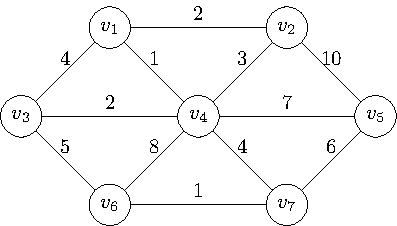
\includegraphics[width=0.8\textwidth]{Figure/min_span.pdf}
\end{figure}
\end{minipage}
\begin{minipage}{0.25\textwidth}
\begin{figure}[H]
  \centering
  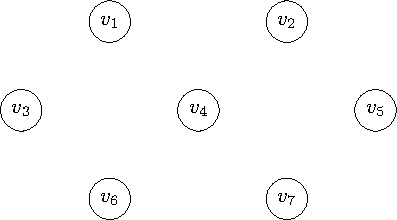
\includegraphics[width=0.8\textwidth]{Figure/Kruskal_algo_d1.pdf}
\end{figure}
\end{minipage}
\begin{minipage}{0.25\textwidth}
\begin{figure}[H]
  \centering
  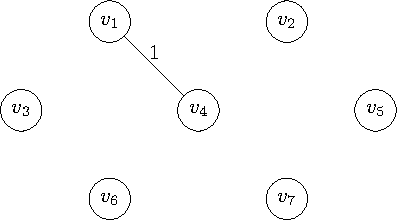
\includegraphics[width=0.8\textwidth]{Figure/Kruskal_algo_d2.pdf}
\end{figure}
\end{minipage}
\begin{minipage}{0.25\textwidth}
\begin{figure}[H]
  \centering
  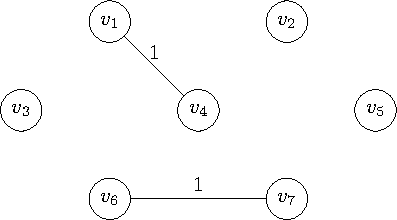
\includegraphics[width=0.8\textwidth]{Figure/Kruskal_algo_d3.pdf}
\end{figure}
\end{minipage}

\begin{minipage}{0.25\textwidth}
\begin{figure}[H]
  \centering
  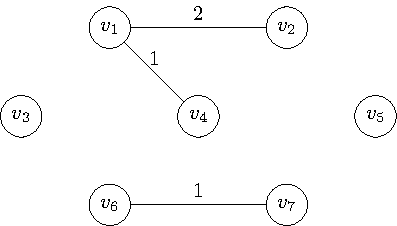
\includegraphics[width=0.8\textwidth]{Figure/Kruskal_algo_d4.pdf}
\end{figure}
\end{minipage}
\begin{minipage}{0.25\textwidth}
\begin{figure}[H]
  \centering
  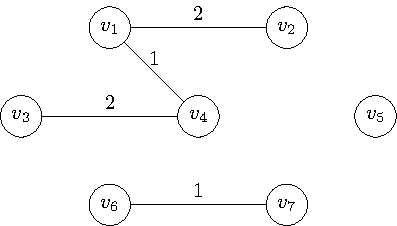
\includegraphics[width=0.8\textwidth]{Figure/Kruskal_algo_d5.pdf}
\end{figure}
\end{minipage}
\begin{minipage}{0.25\textwidth}
\begin{figure}[H]
  \centering
  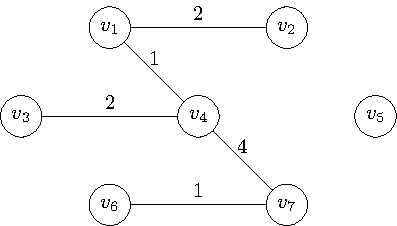
\includegraphics[width=0.8\textwidth]{Figure/Kruskal_algo_d6.pdf}
\end{figure}
\end{minipage}
\begin{minipage}{0.25\textwidth}
\begin{figure}[H]
  \centering
  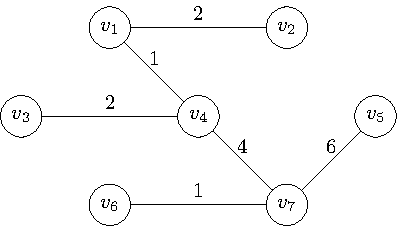
\includegraphics[width=0.8\textwidth]{Figure/Kruskal_algo_d7.pdf}
\end{figure}
\end{minipage}

This algorithm terminates when enough edges have been accepted to form a spanning tree. It is simple to decide whether an edge \((u, v)\) should be accepted or rejected. The appropriate data structure for making this decision is the \emph{union-find} (or disjoint-set) algorithm. The key invariant is that, at any point in the process, two vertices belong to the same set if and only if they are connected in the current spanning forest.

Initially, each vertex is placed in its own set. If \(u\) and \(v\) are found to be in the same set, the edge \((u, v)\) is rejected, since adding it would form a cycle. Otherwise, the edge is accepted, and a union operation is performed on the two sets containing \(u\) and \(v\).

The worst-case running time of this algorithm is \(O(\vert E \vert \log \vert E \vert)\), dominated by the heap operations required for edge sorting. Since \(\vert E \vert = O(\vert V \vert^2)\), this time complexity simplifies to \(O(\vert E \vert \log \vert V \vert)\). In practice, the algorithm performs significantly faster than this theoretical bound might suggest.

\section{Depth-First Search}
Depth-First Search (DFS) is a generalization of pre-order traversal. Starting at some vertex \(v\), we process \(v\) and then recursively traverse all vertices adjacent to \(v\). If this process is performed on a tree, then all tree vertices are systematically visited in a total of \(O(\vert E \vert)\) time.

If we perform this process on an arbitrary graph, we need to be careful to avoid cycles. To do this, when we visit a vertex \(v\), we mark it as visited to indicate that we have already been there, and then recursively call depth-first search on all adjacent vertices that are not already marked.
